\chapter{Progettazione} % Main chapter title

\label{Capitolo4} % For referencing the chapter elsewhere, use \ref{Chapter1} 

\lhead{Capitolo 4. \emph{Progettazione}} % This is for the header on each page - perhaps a shortened title

Molto spesso, non si progetta una struttura che reagisca in maniera elastica ma coerente alle modifiche.
Ad aggravare la situazione, i cambiamenti effettuati non sempre sono documentati per cui le specifiche non vengono aggiornate e ciò rende i cambiamenti futuri difficili da compiere. Conscio di tale realtà, si è cercato di progettare il sistema tenendo in mente le possibili evoluzioni.

\section{Architettura}

La documentazione Android non definisce dei pattern architetturali da seguire, e non rende semplice sviluppo di pattern noti (view e controller sono fortemente accoppiati). Inoltre la filosofia delle API è incentrata sulla derivazione piuttosto che sulla composizione, il che rende anche difficile fare dei test accurati.

Le linee guida di Google per gli sviluppatori indicano che è necessario:

\begin{itemize}
\item Definire la UI (User Interface) in diversi XML in base alla risoluzione e all'hardware
\item Definire le risorse in altri XML
\item Estendere classi come ListActivity,TabActivity e utilizzare i sopracitati XML attraverso l'uso di inflaters
\item Creare le classi desiderate per la Business Logic
\end{itemize}


Vengono definiti i seguenti 7 Packages:

\begin{itemize}
\item Activity
\item Service
\item DataModel
\item Core
\item Social
\item Util
\item Adapter
\end{itemize}

\subsection{Package Activity}

L'activity è uno dei 4 elementi di base che vanno a costituire un'applicazione:

\begin{itemize}
\item Activity
\item Broadcast Intent Receiver
\item Service
\item Content Provider
\end{itemize}

La classe Activity è uno degli elementi centrali di ogni applicazione Android. L'Activity è un concetto legato allo sviluppo delle interfacce grafiche: normalmente una Activity rappresenta una singola schermata della nostra applicazione. Le applicazioni possono definire una o più Activity per trattare diverse fasi del software: ogni Activity è responsabile del salvataggio del proprio stato in modo da poterlo ristabilire successivamente come parte del ciclo di vita dell'applicazione.
Ci può essere solo una Activity attiva per volta, quindi una sola Activity per volta può essere in “primo piano” nello stesso tempo: una che in un determinato momento non si trova nello stato attivo e quindi non si trova in foreground potrebbe essere terminata dal sistema operativo ad esempio perché la memoria diventa insufficiente. Questo significa che ogni applicazione Android può cambiare lo stato in ogni momento e deve essere pronta ad essere interrotta e chiusa in ogni istante.

A seguire il modello di ciclo di vita di una Activity:

\begin{figure}[h]\centering  
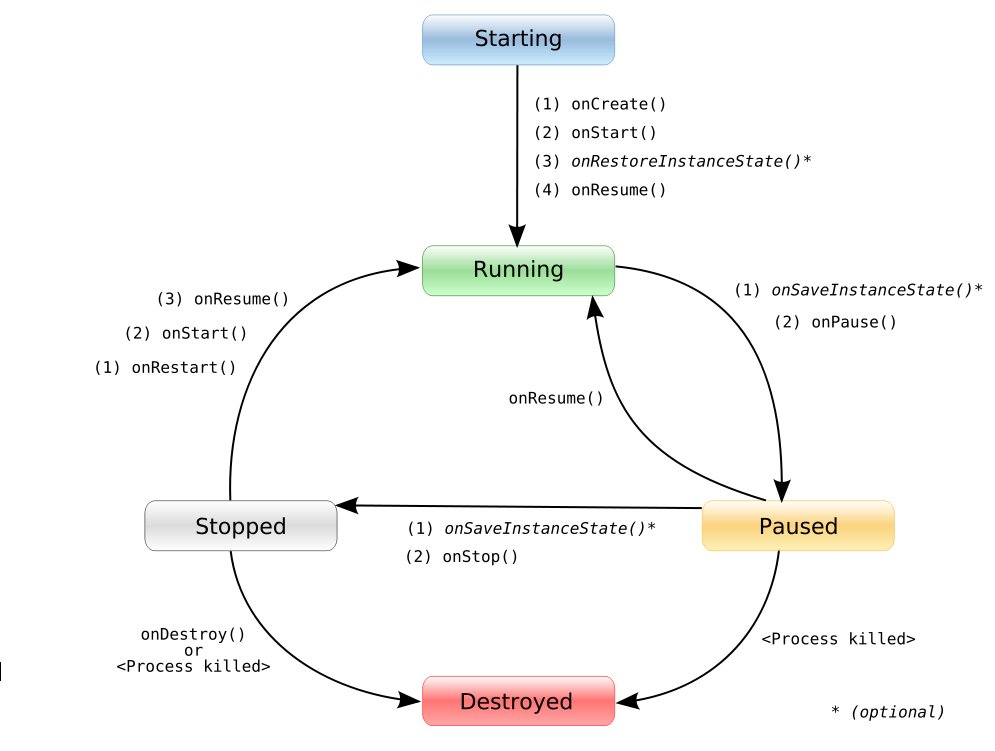
\includegraphics[scale=0.38]{/workspace/1911_up/Dropbox/thesis/Figures/ciclovitaattivita.jpg}
\caption[Long caption]{Caption}
\label{pic-a}
\end{figure}

L'attività richiesta in tale progetto consiste in una view che permetta di mandare a schermo i fotogrammi registrati dalla fotocamera ed altre informazioni d'uso. Essa deve inoltre registrare tutte le informazioni utili quali gli input utente.

Vengono quindi definite le seguenti Activity:
\begin{itemize}

\item \textbf{Activity::FaceDetectionBase}

\textit{Estende:} Activity.

\textit{Descrizione ed utilizzo:} Definisce gli elementi comuni alle activity \textit{Activity::FaceDetectionActivity} e \textit{Activity::StaticFaceDetectionActivity}.


\item \textbf{Activity::FaceDetectionActivity}

\textit{Estende:} Activity::FaceDetectionBase.

\textit{Implementa:} CvCameraViewListener2.

\textit{Descrizione ed utilizzo:} Attività poggiata su un subclassing di una classe di OpenCV dedita al riconoscimento di oggetti. Consente il rilevamento facciale e deve permettere di riconoscere le parti facciali richieste. Deve permettere di ricavare l'orientamento del volto in base alle fattezze del triangolo descritto dalla giunzione tra occhi e bocca.

\item \textbf{Activity::StaticFaceDetectionActivity}

\textit{Estende:} Activity::FaceDetectionBase.

\textit{Descrizione ed utilizzo:} Simile a FaceDetectionActivity, ma la sua funzione è statica, ossia l'eventuale rilevamento si basa su immagini statiche inserite dall'utente (scattate al momento o caricate direttamente dallo smartphone).

\item \textbf{Activity::PhotoActivity}

\textit{Estende:} Activity.

\textit{Descrizione ed utilizzo:} Attività che permette di salvare l'eventuale fotografia scattata e di condividerla attraverso mail,servizi di messaggistica e Facebook.

\item \textbf{Activity::ErrorHandlerActivity}

\textit{Estende:} Activity.

\textit{Descrizione ed utilizzo:} classe dedicata alla segnalazione degli errori. Ogni qual volta venga lanciata un'eccezione, questa verrà gestita ed inoltrata ad un'activity dedicata che possa fornire allo sviluppatore il log completo dell'errore (direttamente all'interno dell'applicazione senza il bisogno di controllare il Logcat). Sarà possibile attraverso un apposito botto tornare alla sezione che ha causato il crash per appurarne le dinamiche.


\item \textbf{Activity::TutorialActivity}

\textit{Estende:} Activity.

\textit{Descrizione ed utilizzo:} Attività contenente un tutorial illustrativo che si prefigge di rendere chiaro l'utilizzo dell'applicazione.

\item \textbf{Activity::SplashScreenActivity}

\textit{Estende:} Activity.

\textit{Descrizione ed utilizzo :}Questa attività raccoglie semplicemente l'animazione del logo dell'azienda e deve permettere all'utente di scegliere se effettuare il login sul social network Facebook (opzionale per il proseguimento) ed inoltre permettere di accedere al programma previo accettazione dei termini di servizio.

\end{itemize}
\subsection{Package Service}

Un Service è un processo che lavora in background senza la diretta interazione con l'utente (un concetto molto simile al deamon in ambiente Unix). La classe Service viene utilizzata per creare componenti software che possono svolgere attività in modo “invisibile”, senza interfaccia utente. Utilizzando i Service è possibile gestire le nostre applicazioni e farle reagire ad eventi anche quando non sono in primo piano: un Service può essere avviato, fermato e controllato da altri componenti dell'applicazione, inclusi altri Service e Activity. Nello specifico tale strumento viene utilizzato per gestire eventuali chiamate al WebServer aziendale (richiesta di aggiornamento, sistema di notifiche).

Vengono così definite le classi:
\begin{itemize}


\item \textbf{Service::BootStartUpReceiver}

\textit{Estende:} BroadcastReceiver

\textit{Descrizione ed utilizzo:} Classe dedita esclusivamente all'avvio del Service indicato. E' possibile, tramite un particolare flag nel file \textit{Manifest.xml}, definire quando avviare tale servizio.

\item \textbf{Service::BackgroundService}

\textit{Estende:} Service. 

\textit{Descrizione ed utilizzo:} Classe che rappresenta il service dedito condivisione dei contenuti.
\end{itemize}

\subsection{Package Model}

Tale package è stato definito al fine di scindere il più possibile la parte puramente grafica dal modello.

Di seguito le classi definite:
\begin{itemize}

\item \textbf{Model::Data}

\textit{Estende:} nessuna classe.

\textit{Descrizione ed utilizzo:} Classe contenente i risultati degli input utente.

\item \textbf{Model::Sprite}

\textit{Estende:} nessuna classe.

\textit{Descrizione ed utilizzo:} Classe di diagnostica per il testing visuale dell'applicazione. Contiene i dati grezzi dei risultati ottenuti.

\end{itemize}
\subsection{Package Core}

\begin{itemize}
\item \textbf{Core::Camera}

\textit{Estende: JavaCameraView (OpenCV)}

\textit{Descrizione ed utilizzo:}permette la modifica dei parametri OpenCV a runtime quali risoluzione, profondità minima e massima di campionamento, numero di volti individuati necessari per la validazione, selezione della camera da utilizzare, etc.

\item \textbf{Core::Templates}

\textit{Estende:} nessuna classe. 

\textit{Descrizione ed utilizzo:} Classe contente funzioni che operano sui templates per il rilevamento del volto e delle parti richieste.
\end{itemize}
\subsection{Package Social}

Tale package contiene le classi:
\begin{itemize}
\item \textbf{Social::LoginSession}

\textit{Estende:} nessuna classe.

\textit{Descrizione ed utilizzo:} Classe che permette all'utente di effettuare l'accesso al social network Facebook e di mantenere la sessione di login attiva fino alla scadenza del token di validità.

\item \textbf{Social::Share}

\textit{Estende:} nessuna classe.

\textit{Descrizione ed utilizzo:} Classe adibita alla pubblicazione dei contenuti multimediali eventualmente creati.
\end{itemize}

\subsection{Package Utility}
Contiene le seguenti classi:

\begin{itemize}

\item \textbf{Utility::MatUtils}

\textit{Estende:} nessuna classe.

\textit{Descrizione ed utilizzo:} Classe generica per operazioni su oggetti appartenenti alla classe OpenCV Mat.

\item \textbf{Utility::Generics}

\textit{Estende:} nessuna classe.

\textit{Descrizione ed utilizzo:} Classe generica contenente principalmente funzioni statiche utilizzate per varie operazioni all'interno dell'applicazione.
\end{itemize}


\subsection{Package Adapter}
Contiene le seguenti classi:

\begin{itemize}

\item \textbf{Adapter::CustomAdapter}

\textit{Estende:} BaseAdapter.

\textit{Descrizione ed utilizzo:} Classe la cui instanza viene utilizzata per il caricamento di dati grezzi all'interno della ListView (utilizzata per la scelta degli Sprite o delle applicazioni disponibili per la condivisione).

\end{itemize}

\section{Dettagli in fase di codifica}

\textbf{1:} Essendo una applicazione che lavora principalmente in real-time, particolare attenzione è stata dedicata alla creazione di oggetti dinamici (in modo da evitare rallentamenti dovuti all'azione di pulizia del \textit{Garbage Collector})

\textbf{2:} Normalmente per la fruizione delle librerie OpenCV è necessario installare all'interno del dispositivo l'applicazione OpenCV Manager, che si occupa di precaricare le librerie e di renderle disponibili. Data la scomodità di tale soluzione, si è preferito compilare le librerie senza il Manager ed aggiungerle staticamente direttamente nell'applicazione.

\newpage

\section{Associazione Classi-Requisiti}

Di seguito viene indicata la mappatura Classi$\rightarrow$ Requisiti.

\begin{center}
    \begin{longtable}{| p{6cm} | p{2cm} |}
    \hline
    Classe & Requisito \\ \hline
     Activity::FaceDetectionActivity & RFO1.1  \\ \hline
     Core::Templates & RFO1.1 \\ \hline
     Utility::MatUtils & RFO1.1 \\ \hline
     Core::Camera & RFO1.2.1 \\ \hline
     Core::Camera & RFO1.2.2\\ \hline
     Core::Camera & RFO1.2.3  \\ \hline
     Core::Camera & RFO1.2.4 \\ \hline
     Core::Camera & RFO1.2.5\\ \hline
     Core::Camera & RFO1.2.6\\ \hline
     Core::Camera & RFO1.2.7 \\ \hline
     Activity::FaceDetectionActivity & RFD1.3 \\ \hline    
	 Model:Sprite & RFO1.4.1 \\ \hline
     Adapter::CustomAdapter & RFO1.4.2  \\ \hline
     Utility::Generics & RFO1.4.3 \\ \hline
     Activity::StaticFaceDetectionActivity & RFO2.1 \\ \hline
     Activity::StaticFaceDetectionActivity & RFO2.2\\ \hline
	 Model:Sprite & RFO2.3 \\ \hline
     Adapter::CustomAdapter & RFO2.3  \\ \hline
     Utility::MatUtils & RFD3.1 \\ \hline
     Activity::PhotoActivity & RFD3.2.1   \\ \hline
     Activity::PhotoActivity & RFD3.2.2  \\ \hline
     Service::BootStartUpReceiver & RFD3.2.2 \\ \hline
     Service::BackGroundService  & RFD3.2.2 \\ \hline
     Activity::PhotoActivity & RFD3.2.3 \\ \hline    
     Social::LoginSession & RFD3.3.1 \\ \hline
     Social::Share & RFD3.3.2 \\ \hline
     Social::Share & RFD3.3.3\\ \hline
     classe non mappata & RFD4  \\ \hline
     Activity::SplashScreenActivity & requisito non mappato  \\ \hline
     Activity::TutorialActivity & requisito non mappato  \\ \hline
    \end{longtable}
\end{center}

I requisiti non mappati corrispondono a richieste dell'azienda avvenute in corso d'opera, posteriori allo studio dell'architettura di sistema.

\section{Tecnologie utilizzate}

\subsection{Java}

Il linguaggio per applicazioni Android è in realtà un "dialetto" del linguaggio Java così come è diversa anche la virtual machine di runtime (Dalvik virtual machine anziché JVM).
In una normale applicazione Android non c'è un entry point (il classico metodo "main") da dove normalmente un programma comincia a caricare le sue parti software e avviarsi: tutto è pensato per essere un "componente" pilotato dagli eventi ("Event Driven") dell'hardware o di altri componenti. Questo paradigma fa sì che il programmatore sviluppi per ogni hardware delle routine il più possibile indipendenti. Un vantaggio è che il sistema operativo potrà ottimizzare le risorse, ad esempio rinunciando a caricare componenti (e hardware) non supportati o non prioritari perché inutilizzati.

\subsection{Android NDK}

L'NDK (Native Development Kit) è uno strumento che permette di implementare parte dell'applicazione usando codice scritto in linguaggio nativo come il C ed il C++. Per alcune applicazioni può essere utile in quanto si può riutilizzare le librerie scritte in tali linguaggi. L'uso di tale strumento non da però beneficio per la maggior parte delle applicazioni ed è da usare quindi con parsimonia (spesso l'aumento delle performance dovuto all'utilizzo di codice nativo non giustifica l'aumento di complessità). Tipicamente buoni candidati sono programmi che sono CPU-intensive che non allocano molta memoria come simulazioni fisiche ed analisi dei segnali. Nel caso specifico sono stati effettuati dei test per verificare se la quantità di chiamate verso la libreria C/C++ OpenCV giustifica tale strumento. Tale libreria è stata utilizzata per prototipi usa e getta ed è stata successivamente scartata su richiesta dell'azienda.

\subsection{Android Studio}

Basato su IntelliJ IDEA, Android Studio è un ambiente di sviluppo integrato (IDE) specifico per la piattaforma Android. Esso fornisce strumenti molto potenti come lo smart editing, re-fattorizzazione del codice, layout editor, supporto a Gradle, supporto a Maven. Contiene al suo interno le SDK. Infatti le applicazioni di Android sono sviluppate all'interno di un framework, una struttura dati specifica che comprende un vasto set di strumenti di sviluppo come:

\begin{itemize}
\item Debugger
\item Dalvik Debug Monitor Server (DDMS)
\item Librerie Android
\item Emulatore basato su QEMU
\item Documentazione
\end{itemize}

\subsection{Android FD-Library}

All'interno delle SDK Android è presente una API per il riconoscimento facciale: Android.Media.FaceDetector. Questa classe permette, data un immagine, di trovare le eventuali facce presenti attraverso il semplice utilizzo del metodo findFaces(). Ogni istanza ritornata viene salvata in un array Faces[] e contiene:

\begin{itemize}
\item Valutazione se si tratta di un volto o meno 
\item Distanza tra gli occhi (numero di pixel)
\item Posizione (x,y) del punto medio situato tra i due occhi
\item Rotazioni di posa della faccia (x,y,z)
\end{itemize} 

A seguito di valutazioni e di un prototipo usa e getta si è però deciso di non utilizzare in quanto:

\begin{itemize}
\item Non ritorna il rettangolo che include con precisione la faccia

\item Non consente di utilizzare template a piacimento per la ricerca di parti specializzate (naso, occhi, orecchie, etc.)

\item Prestazioni buone per immagini singole, ma non adatta ad un applicazione real-time

\item Sono stati rilevati comportamenti evidentemente diversi a seconda del dispositivo utilizzato

\item Quantità non indifferente di bug riportata dalla comunità di sviluppatori Android
\end{itemize}

\subsection{OpenCV}

OpenCV è una libreria creata da Intel a scopi di commerciali e di ricerca. E' una libreria open e gratuita, e pertanto il suo codice può essere utilizzato nella sua interezza o in parte. Al momento della stesura di questo documento la versione più recente disponibile è la v2.4.7 specifica per dispositivi Android. Tale versione fornisce un wrapper Java alle librerie OpenCV che fornisce quasi tutte le fonzionalità core. Al fine di garantire il funzionamento di applicativi basati su questa libreria è però necessario installare sul dispositivo un software chiamato OpenCV Manager, che permette all'applicazione ottimizzazioni in base all'hardware presente.

Vi sono due modi d'utilizzo di questa libreria:

\begin{itemize}
\item \textbf{Ad alto livello}:  utilizzo esclusivo delle Java API. Facilità di sviluppo, ma non permette l'accesso completo alle libreria. Prestazioni minori a causa al gran numero di chiamate JNI (Java Native Interface) verso la libreria

\item \textbf{A basso livello}:  utilizzo dell'interfaccia nativa di openCV. Android permette infatti di eseguire chiamate a funzioni native, ciò significa che è possibile utilizzare l'interfaccia C++ di OpenCV. 
\end{itemize}
%----------------------------------------------------------------------------------------
\subsection{GenyMotion}

Genymotion è un emulatore Android alternativo disponibile per Windows, Mac e Linux. Verrà utilizzato al posto dell'emulatore proprietario di Android Studio per le sue doti velocistiche che permettono una non indifferente riduzione dei tempi di sviluppo.

\subsection{JTest}

JTest è una suite completa di strumenti per l'analisi statica del codice Java dal momento che fornisce molte informazioni sulle metriche (ne misura la complessità), individuando in esso i punti critici e facilitando così lo sviluppo del codice (che deve rispettare le norme assegnate). Facilita inoltre la review del codice, permette test d'unità e tracciamento di errori a tempo di esecuzione. E' lo strumento utilizzato dall'azienda ospitante lo stage, pertanto è di vincolo utilizzare tale sistema per il test dell'applicazione.


\subsection{Doxygen}

Doxygen è un tool per la generazione di documentazione di sorgenti di vario genere, compresi quelli Java. Esso si basa su un file di configurazione che contiene le numerose opzioni configurabili messe a disposizione per la generazione della documentazione. Inoltre supporta l'esportazione, tra le tante,
dei documenti sia in HTML che in LATEX. Nel progetto è stato utilizzato per la generazione di tutta la documentazione ottenibile dal codice in maniera automatica.

\subsection{Subversion}

Il sistema di controllo di versione utilizzato dall'azienda è SVN, pertanto è di vincolo utilizzare tale sistema per il versionamento dell'applicazione.


%----------------------------------------------------------------------------------------
\newpage
\section{Problematiche}

\subsection{Riduzione complessità}

Al fine di garantire un facile utilizzo della libreria Java OpenCV, sono state creati alcuni metodi con l'obbiettivo di suddividere il problema in sotto-problemi più semplici e facili da gestire e manutenere. L'intero rilevamento facciale e delle sue componenti viene gestito da un'unica funzione di dimensioni modeste:

\begin{lstlisting}
	public Mat onCameraFrame(CvCameraViewFrame inputFrame) {
		
		Mat equalizedGrayMat = MatUtils.equalize(inputFrame.gray());
		MatOfRect faces = new MatOfRect();
		
		mSelectedDetector.detectMultiScale(equalizedGrayMat, 
						faces, 
						mScaleFactor,
					        mMinNeighbors,
						mFlags, 
						mMinSize,
						mMaxsize);
						
		Rect[] facesArray = faces.toArray();

		for (int i = 0; i < facesArray.length; i++) {
			
			Rect r = facesArray[i];
			Rect eyearea = getEyesArea();
			Rect eyearea_right = getRightEyeRect(eyearea);
			Rect eyearea_left = getLeftEyeRect(eyearea);
			Rect nose_area = getNoseRect(getNoseROI(r, eyearea));
			Rect mouth_area = getMouthRect(getMouthROI(r, nose_area));

			if (mMust_Learn) {
				teplateER = create_new_template(mJavaDetectorEye, inputFrame.RGBA(), eyearea_right, 24, 1);
				teplateEL = create_new_template(mJavaDetectorEye, inputFrame.RGBA(), eyearea_left, 24, 1);
				teplateN = create_new_template(mJavaDetectorNose, inputFrame.RGBA(), nose_area, 24, 0);
				teplateM = create_new_template(mJavaDetectorMouth, inputFrame.RGBA(), mouth_area, 24, 0);
				.
				.
				//creazione di templates di interesse aggiuntivi
			} else {
			    match_feature(eyearea_right, teplateER, 1);
				match_feature(eyearea_left, teplateEL 1);
				match_feature(nose_area, teplateN, 2);
				match_feature(mouth_area, teplateM, 3); 
				.
				.
				//matching di templates di interesse aggiuntivi
			}
		}
\end{lstlisting}

Dove, sequenzialmente:
\begin{itemize}
\item il frame immagine in ingresso viene desaturato per ridurre la quantità di informazioni inoltrate, dal momento che l'algoritmo OpenCV lavora indipendentemente dai colori presenti. L'equalizzazione è invece necessaria per compensare le variazioni di luminosità nelle varie parti dell'immagine
\item la funzione \textit{detectMultiScale$(Mat ...)$} rileva i volti presenti e li immagazzina all'interno di un array (ne salva il rettangolo contenente il volto individuato)
\item per tutti gli elementi dell'array:
\begin{itemize}
\item ricava la regione d'interesse corrispondente alla feature da cercare (partendo dal presupposto che ogni feature facciale ha una posizione approssimabile statisticamente)
\item se viene richiesta la creazione di un template:
\begin{itemize}
\item crea un template grazie a un classificatore che lavora nella regione di interesse indicata in base al tipo della feature
\end{itemize}
\item altrimenti:
\begin{itemize}
\item esegue il template matching nella regione di interesse indicata
\end{itemize}
\end{itemize}
\end{itemize}

La prima funzione presa in analisi è \textit{redo\_template$(...)$} che trova la parte desiderata nella regione di interesse (ROI) indicata. 
Tale regione è stata ricavata da una stima statistica dell'altezza delle varie parti rispetto al volto ed è necessaria per ridurre al minimo il costo computazionale di ricerca delle singole parti. 

\begin{lstlisting}
    private void create_new_template(CascadeClassifier classificator, Mat source , Rect roi, boolean isEye) {
        Mat template = new Mat();
        Mat mROI = source.submat(roi);
        MatOfRect feature = new MatOfRect();
        Point iris = new Point();
        Rect feature_template = new Rect();
        classificator.detectMultiScale(mROI, feature, 1.15, 2,
                Objdetect.CASCADE_FIND_BIGGEST_OBJECT
                        | Objdetect.CASCADE_SCALE_IMAGE, new Size(30, 30),
                new Size());
 
        Rect[] eyesArray = feature.toArray();
        for (int i = 0; i < eyesArray.length;) {
            Rect e = eyesArray[i];
            e.x = area.x + e.x;
            e.y = area.y + e.y;
            Rect feature_rectangle = new Rect((int) e.tl().x,
                    (int) (e.tl().y + e.height * 0.4), (int) e.width,
                    (int) (e.height * 0.6));
            .
            .            
 \end{lstlisting} 
 
Di particolare valore è il metodo \textit{detectMultiScale(const Mat image, vector<Rect> objects, double scaleFactor, int minNeighbors, int flags, Size minSize, Size maxSize)} chiamato dal classificatore dove i parametri:
 \begin{itemize}
 \item \textit{scaleFactor}: indica di quanto la dimensione dell'immagine è ridotta ad ogni scaling. Si crea quindi una piramide di immagini in cui l'immagine in posizione k è di dimensioni inferiori all'immagine in posizione k-1. Maggiore sarà questo valore, minore sarà il costo computazionale ma lo sarà anche il rate di rilevamento.

\begin{figure}[h]\centering  
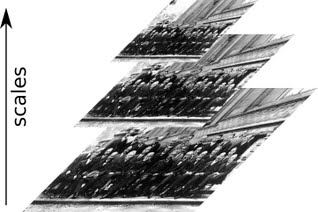
\includegraphics[scale=0.8]{/workspace/1911_up/Dropbox/thesis/Figures/pyramid.jpg}
\caption[Image Pyramid]{Image Pyramid}
\label{pic-a}
\end{figure} 

\item \textit{Image}: immagine di input, preferibilmente desaturata ed equalizzata.

\item \textit{objects}: vettore all'interno del quale saranno inseriti i rettangoli contenenti i volti individuati.

\item \textit{minNeighbors}: indica la qualità dei volti rilevati. Maggiore sarà tale parametro, maggiore sarà la precisione ma con il rischio che anche i volti corretti siano scartati.

\item \textit{flags}: indicano specifiche condizioni che il classificatore deve seguire (come ad esempio saltare alcune regioni o cercare l'oggetto di dimensioni massime).

\item \textit{minSize}: Dimensione minima degli oggetti, sotto la quale vengono ignorati.

\item \textit{maxSize}: Dimensione massima degli oggetti, oltre la quale vengono ignorati.
 
\end{itemize}
 
Nel caso l'input al metodo richieda di trovare l'occhio e in particolare la pupilla, riduco la regione di interesse e grazie alla funzione OpenCV \textit{Core.minMaxLoc(...)} è possibile trovare il punto più scuro dell'occhio (ossia la pupilla). 

Successivamente per questioni di verifica disegna sulla sottomatrice Mat il rettangolo contenente l'occhio e il cerchio contenente la pupilla.\\
         
\begin{lstlisting}    
                .    
                .
                mROI = source.submat(feature_rectangle);
                Mat vyrez = sourceRGBA.submat(feature_rectangle);
               
  	            Core.MinMaxLocResult darkPoint = Core.minMaxLoc(mROI);
            
 	            Core.circle(vyrez, darkPoint.minLoc, 2, new Scalar(255, 255, 255, 255), 2);
	            iris.x = darkPoint.minLoc.x + feature_rectangle.x;
 	            iris.y = darkPoint.minLoc.y + feature_rectangle.y;
	            feature_template = new Rect((int) iris.x - size / 2, (int) iris.y
	                    - size / 2, size, size);
	            Core.rectangle(sourceRGBA, feature_template.tl(), feature_template.br(),
 	                   new Scalar(255, 0, 0, 255), 2);
	            template = (source.submat(feature_template)).clone();
            }
            return template;
        }
        return template;
    }
\end{lstlisting}

Una volta creato il template, per i frame successivi verrà utilizzato \textit{match\_feature$(...)$} che appunto utilizza il template creato da \textit{create\_new\_template$(...)$}. 

Il template matching utilizzato per mezzo del metodo OpenCV \textit{$matchTemplate(...)$} non è basato su istogrammi ma è basato sul match di un template che viene fatto "scivolare" contro un'immagine di input.\\

\begin{figure}[H]\centering  
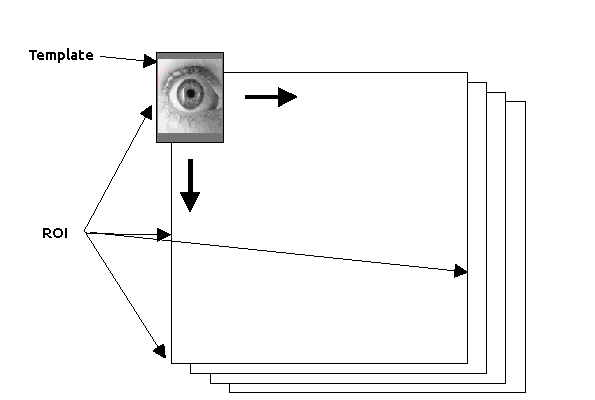
\includegraphics[scale=0.8]{/workspace/1911_up/Dropbox/thesis/Figures/slide.png}
\caption[Sliding Template Matching]{Sliding Template Matching}
\label{pic-a}
\end{figure}

\begin{lstlisting}
private void match_feature(Rect roi, Mat template, int type) {
        Point matchLoc;
        Mat ROI = mGray.submat(roi);
        int result_cols = mROI.cols() - template.cols() + 1;
        int result_rows = mROI.rows() - template.rows() + 1;
		
        Mat mResult = new Mat(result_cols, result_rows, CvType.CV_8U);
 
        Imgproc.matchTemplate(ROI, mTemplate, mResult,Imgproc.TM_CCORR_NORMED);
 
        Core.MinMaxLocResult mmres = Core.minMaxLoc(mResult);
		.
		.
		.
    }
\end{lstlisting}

Come si può vedere dalla funzione è stato utilizzato il metodo TM\_CCORR\_NORMED nella regione di interesse ROI. 

Utilizzando \textit{I} per denotare l'immagine in ingresso, \textit{T} per il template si definisce il metodo CV\_TM\_CCORR (Correlation matching method) come: 

\begin{figure}[H]\centering  
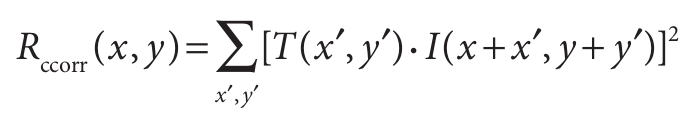
\includegraphics[scale=0.3]{/workspace/1911_up/Dropbox/thesis/Figures/rcor.png}
\caption[Correlation matching method formula]{Correlation matching method formula}
\label{pic-a}
\end{figure}

Dal momento che il template viene moltiplicato contro l'immagine, un match perfetto risulterà grande mentre un match cattivo sarà molto piccolo e tendente a 0.

Di tale metodo ne esiste una versione normalizzata che è utile perchè può ridurre gli effetti di differenze di luce tra l'immagine in ingresso ed il template utilizzato. Il coefficiente di normalizzazione viene definito come:

\begin{figure}[H]\centering  
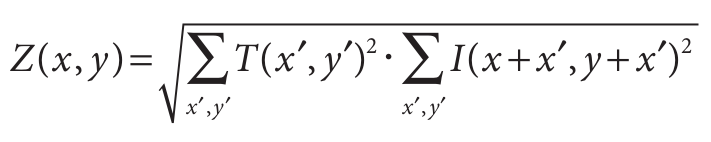
\includegraphics[scale=0.3]{/workspace/1911_up/Dropbox/thesis/Figures/z.png}
\caption[Coefficiente normalizzato]{Coefficiente normalizzato}
\label{pic-a}
\end{figure}

Si definisce infine il metodo CV\_TM\_CCORR\_NORMED come:

\begin{figure}[H]\centering  
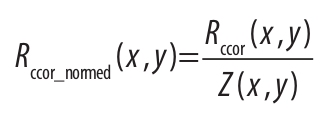
\includegraphics[scale=0.38]{/workspace/1911_up/Dropbox/thesis/Figures/rccor.png}
\caption[Correlation matching method formula (normed)]{Correlation matching method formula (normed)}
\label{pic-a}
\end{figure}

Vi sono anche metodi basati sulla differenza di quadrati ma si è preferito utilizzare dei metodi piu sofisticati in quanto assicurano risultati migliori (tenendo conto della bassa qualità dei fotogrammi in entrata dovuta a fotocamere con sensori ridotti). 

Per aumentare le prestazioni dei sistema sono state effettuate alcune considerazioni a partire dalla meccanica delle librerie OpenCV.

		\begin{figure}[H]\centering  
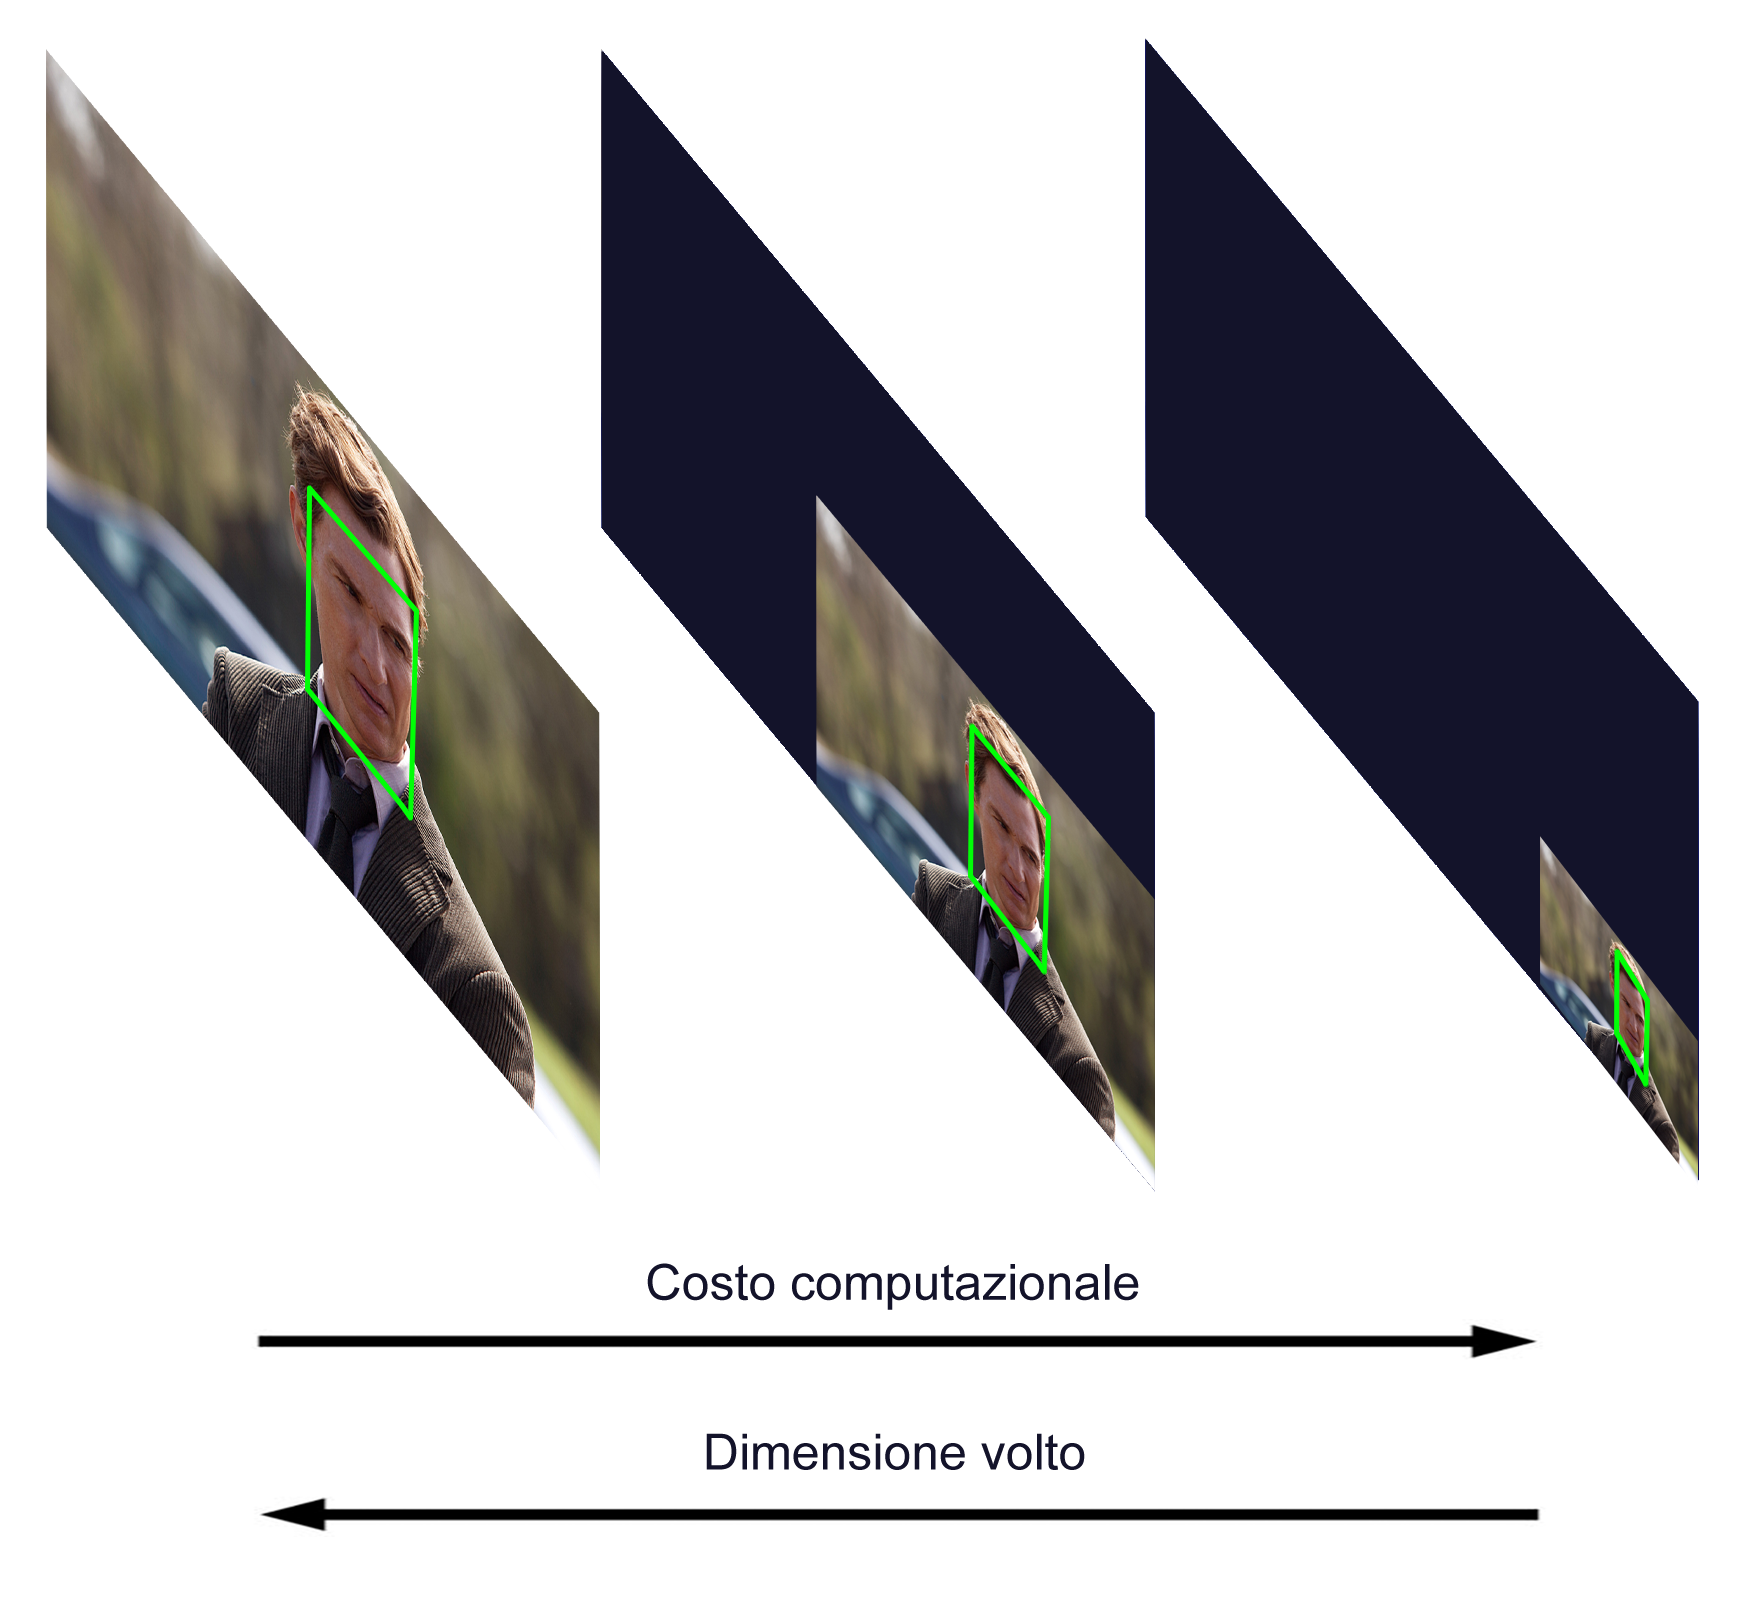
\includegraphics[scale=0.7]{/workspace/1911_up/Dropbox/thesis/Figures/scala.png}
\caption[Costo computazionale al variare della dimensione del volto]{Costo computazionale al variare della dimensione del volto}
\label{pic-a}
\end{figure}

	Dal momento che ogni singolo frame viene valutato nella sua interezza da un classificatore si è deciso di:

	\begin{itemize}
	\item Effettuare ogni \textit{X} millisecondi uno scan completo fino alla massima profondità in modo da rilevare eventuali nuovi volti.
	\item Se sono stati rilevati nuovi volti allora:
	 	\begin{itemize}
			\item Fisso una nuova profondità massima di scan.
		\end{itemize}
	\item Altrimenti:
		\begin{itemize}
			\item Utilizzo la medesima profondità massima di scan.
		\end{itemize}
	\end{itemize}
	

	Inoltre, se per \textit{Z} millisecondi non vi sono volti nuovi, l'area di ricerca si ridurrà dinamicamente fino a corrispondere al K per cento (K>110 per compensare le naturali oscillazioni della testa) della dimensione dell'ultimo volto rilevato (e sarà centrata sullo stesso centro).
	
			\begin{figure}[H]\centering  
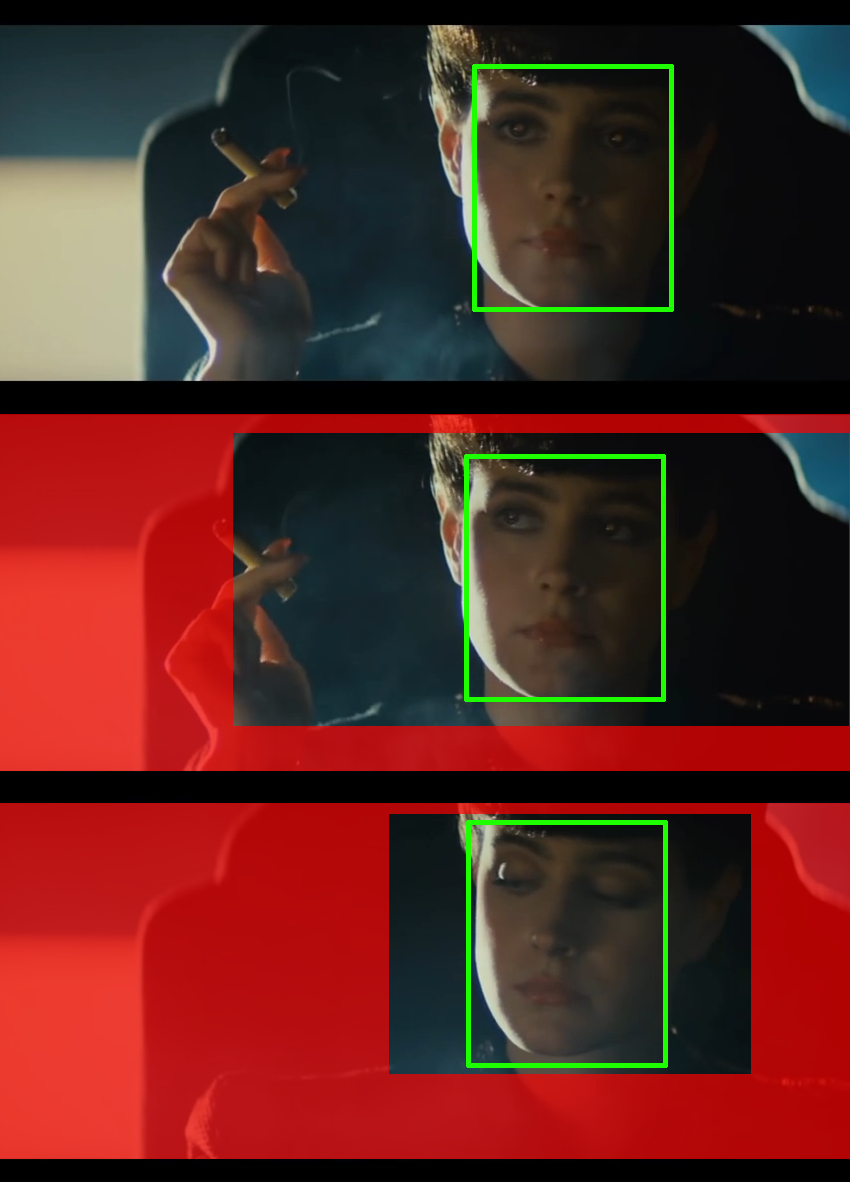
\includegraphics[scale=0.25]{/workspace/1911_up/Dropbox/thesis/Figures/tempo2.png}
\caption[Variazione dinamica della ROI in base alla fedeltà]{Variazione dinamica della ROI in base alla fedeltà}
\label{pic-a}
\end{figure}
	
	In tal modo si permette di migliorare notevolmente le prestazioni (nello specifico più il volto sarà vicino alla camera più il sistema sarà performante).

	Riassumendo:
	\begin{itemize}
	\item Per ogni frame un classificatore Haar viene utilizzato per il rilevamento il volto
	\item Per ogni sottoinsieme di frames positivi per \textit{X} frames viene utilizzato un classificatore Haar per ricavare un template
	\item Per ogni sottoinsieme di frames positivi per \textit{$N-X$} frames viene effettuato template matching 
	\end{itemize}
	
	\textbf{Perchè non effettuare template matching anche per il volto?}

	La tecnica di template matching ha un costo generalmente molto più basso rispetto all'utilizzo di un classificatore ma:
	
	\begin{itemize}
	\item è fotometricamente molto rigido rispetto alle variazioni di luminosità
	\item è geometricamente troppo rigido per essere valido a seguito di variazioni di forma
	\item non ha alcuna strategia per eventuali rilevamenti sovrapposti
	\end{itemize}

\newpage
\subsection{Stima della posa}

Tale funzionalità nasce dalla necessità di gestire il fotogramma in ingresso in base all'inclinazione ed orientamento del volto dell'utente rispetto alla camera. Come già espresso in precedenza, infatti, la meccanica OpenCV per Android si limita a riconoscere solamente volti quasi perfettamente frontali alla camera. Lo studio effettuato è stato mirato a gestire i casi in cui il volto fosse inclinato. Infatti, ottenuti tali informazioni sulla posa, sarebbe stato possibile capire l'inclinazione del volto e di conseguenza ruotare il fotogramma (a tempo di esecuzione) in ingresso per facilitare il riconoscimento da parte del motore. Dal momento che tale funzionalità doveva essere disponibile su dispositivi mobili, sono state effettuate considerazioni prestazionali (test prototipali avevano evidenziato una notevole diminuzione di performance di sistema aggiungendo al rilevamento facciale principale il riconoscimento di una singola parte). 

Pertanto sono state considerate solamente le seguenti parti:

\begin{itemize}
\item Occhio Sinistro viene ad esso associato la cascata cascade\_eye\_sx (Haar)
\item Occhio Destro viene ad esso associato la cascata cascade\_eye\_dx (Haar)
\item Bocca viene ad esso associato la cascata cascade\_mouth (Haar)
\end{itemize}

Per valutare la fattibilità è stata creata una semplice funzione che imprimesse direttamente sul fotogramma un triangolo i cui vertici corrispondono alle parti sopracitate.

\begin{figure}[H]\centering  
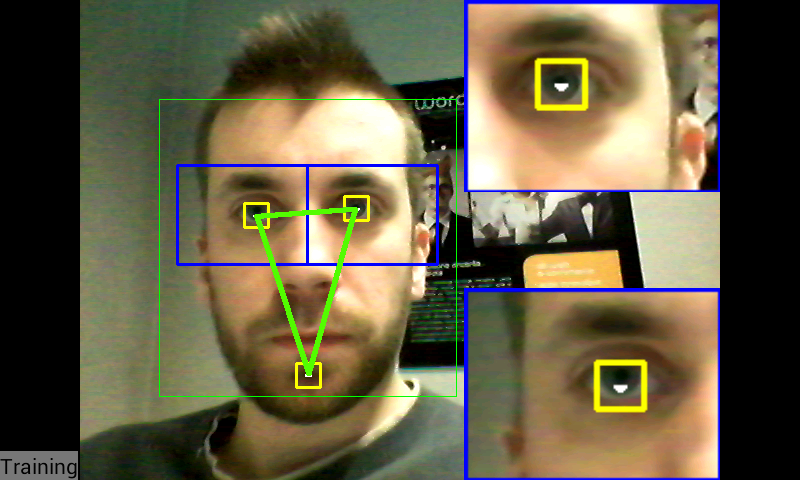
\includegraphics[scale=0.38]{/workspace/1911_up/Dropbox/thesis/Figures/face1_triangle.png}
\caption[Risultato visivo della triangolazione]{Risultato visivo della triangolazione}
\label{pic-a}
\end{figure}

E' stata successivamente creata una funzione che, in base alle fattezze del triangolo, potesse ricavare l'inclinazione del volto. Ottenuti infatti i punti degli occhi, ottengo una retta ed utilizzando della semplice trigonometria trovo l'angolo cercato. A confermare tale cambiamento di rotazione (che viene salvata in un buffer di posizioni) deve essere la posizione della bocca rispetto all'interno del fotogramma.

Dai test effettuati su un prototipo usa e getta sono state evidenziate le seguenti problematiche:

\begin{itemize}
\item La generazione di un template (che avviene ciclicamente ogni secondo per alcuni frame) non garantisce che la posizione della parte trovata coincida con la posizione reale. Se ad esempio la generazione del template avviene un solo occhio è eccessivamente aperto, ci si potrebbe ritrovare in fase di mantenimento ad avere una posizione scorretta fino al successivo evento di generazione template. Quindi, nonostante il volto sia perfettamente frontale, può venire inoltrato al motore OpenCV una richiesta di rotazione della matrice immagine che si traduce in instabilità generale del rilevamento.
\item Le condizioni d'utilizzo (in particolare la luminosità dell'ambiente) possono influire sul risultato: è necessaria quindi un metodo che mantenga la fedeltà del volto individuato per ogni fotogramma. Tale metodo memorizzerà la posizione del rettangolo contenente il volto, la posizione dei rettangoli contenenti occhi e bocca, e le posizioni puntuali di queste ultime parti.
\item Il costo computazionale della creazione dei templates in questo caso è molto elevato e il framerate massimo raggiunto è di 10 fotogrammi al secondo su uno smartphone di fascia alta \textit{(Galaxy S4)}. A questo si aggiunge il costo di rotazione della matrice immagine.
\item Tale approccio può funzionare solo se l'utilizzatore dell'applicazione è unico (non viene gestito il caso in cui la camera trovi più di un volto)
\end{itemize}			

OpenCV fornisce altri strumenti molto potenti come ad esempio \textit{CamShift} ma non è stata possibile un'implementazione a causa dei vincoli temporali sulla tabella di lavoro. Pertanto non è stato possibile eseguire uno studio di fattibilità che potesse risolvere pienamente tale problematica. 


\newpage
\subsection{Memorizzazione volti}

L'applicazione deve essere in grado di rilevare anche più di un volto. Requisito non richiesto ma ritenuto interessante da sviluppare è tenere traccia dei volti.
	Vi possono essere due possibili scenari:
	
	\textbf{Scenario 1:} Applicazione avviata con 2 volti rilevati:
	\begin{itemize}
	\item il primo volto a partire da sinistra sarà identificato come il volto numero 1
	\item il secondo volto a partire da sinistra sarà identificato come il volto numero 2
	\end{itemize}
	
	\textbf{Scenario 2:} Applicazione avviata un solo volto rilevato:
	\begin{itemize}
	\item l'unico volto a partire da sinistra sarà identificato come il volto numero 1
	\item appare un volto a destra del primo, sarà identificato come il volto numero 2
	\end{itemize}
	
	\textbf{Scenario 2 - alternativo:} Applicazione avviata un solo volto rilevato:
	\begin{itemize}
	\item l'unico volto a partire da sinistra sarà identificato come il volto numero 1
	\item appare un volto a sinistra del primo, sarà identificato come il volto numero 1 (mentre il precedente diventerà il numero 2)
	\end{itemize}
	
	Nello scenario alternativo, se una persona provasse degli occhiali in realtà aumentata ma intervenisse nella scena da sinistra un altra persona, perderebbe il "focus" e pertanto gli occhiali verrebbero renderizzati sul volto della seconda persona. 
	
	Per evitare tale scenario, è stata definita una funzione che potesse permettere di "ricordare" posizione e fedeltà dei volti. La fedeltà è necessaria in quanto può capitare che il rilevamento non sia efficace in alcuni frame, e si deve evitare che il render dell'occhiale generi sfarfallii non gradevoli.

